\documentclass[12pt,a4paper,openright, notitlepage]{report}

% l'interlinea
\linespread{1.4}
\setlength{\parskip}{0.3cm plus4mm minus3mm} % spazio verticale paragrafi

\usepackage[italian]{babel} % Italian language
\usepackage[utf8x]{inputenc} % utf8

\usepackage[T1]{fontenc} % Use 8-bit encoding that has 256 glyphs
\usepackage{fourier} % Use the Adobe Utopia font

\usepackage{graphicx}
\usepackage{wrapfig}
\usepackage{subfigure}
\usepackage{changepage}

\usepackage{url}

\usepackage{amsmath,amsfonts,amsthm} % Math packages

\usepackage{sectsty} % Allows customizing section commands
\allsectionsfont{ \normalfont\scshape} % Make all sections centered, the default font and small caps

\usepackage{fancyhdr} % Custom headers and footers
\pagestyle{fancyplain} % Makes all pages in the document conform to the custom headers and footers
\fancyhead{} % No page header - if you want one, create it in the same way as the footers below
\fancyfoot[L]{} % Empty left footer
\fancyfoot[C]{} % Empty center footer
\fancyfoot[R]{\thepage} % Page numbering for right footer
\renewcommand{\headrulewidth}{0pt} % Remove header underlines
\renewcommand{\footrulewidth}{0pt} % Remove footer underlines
\setlength{\headheight}{13.6pt} % Customize the height of the header

\usepackage[font=small,labelfont=bf]{caption} %Style of the caption of figures
\usepackage{float} %to force the figure position

\setlength\parindent{0pt} % Removes all indentation from paragraphs

% Style dell'abstract
\usepackage{abstract}

%----------------------------------------------------------------------------------------
% TITLE
%----------------------------------------------------------------------------------------

\newcommand{\horrule}[1]{\rule{\linewidth}{#1}}

\title{	
\normalfont \normalsize 
\textsc{Università degli studi di Bologna} \\ [25pt]
\horrule{0.5pt} \\[0.4cm]
\huge Visual Directions \\
\horrule{2pt} \\[0.5cm]
}

\author{Andrea Aquino, Matteo Brucato, Miro Mannino}

\date{\normalsize\today}

\begin{document}

\maketitle

\begin{abstract}
Lo scopo del progetto Visual Directions consiste nel semplificare la memorizzazione preventiva di percorsi (principalmente cittadini). Lo stesso è rivolto a chiunque intenda studiare le caratteristiche fondamentali di un percorso tra due punti (non eccessivamente distanti l’uno dall’altro) al fine di poterlo poi percorrere senza l’ausilio di mappe, navigatori o altri mezzi di orientamento. Visual Directions propone due alternative alla visualizzazione dei percorsi fornita dall’applicativo Google Maps. Attraverso una accurata fase di design ed una intensiva fase di testing è stato possibile misurare la resa del progetto in termini di efficienza, efficacia e soddisfazione e confrontare i risultati relativi al fine di stabilire quale delle tre visualizzazioni è da considerarsi la migliore.
\end{abstract}

%----------------------------------------------------------------------------------------
%----------------------------------------------------------------------------------------

\chapter{Introduzione}

Lo scopo del progetto Visual Directions consiste nel semplificare la memorizzazione preventiva di percorsi, principalmente cittadini. Lo stesso è rivolto a chiunque intenda studiare le caratteristiche fondamentali di un percorso tra due punti (non eccessivamente distanti l’uno dall’altro) al fine di poterlo poi percorrere senza l’ausilio di mappe, navigatori o altri mezzi di orientamento. I dati necessari alla memorizzazione di un percorso cittadino sono, ad esempio: punti di svolta, segnaletica stradale, palazzi, scuole, chiese, fontane, semafori, negozi, etc. 

Sistemi come Google Maps e Google Street View permettono, in modi differenti, di visualizzare e memorizzare dei percorsi urbani. Ciononostante, a nostro avviso, non si rivelano particolarmente adatti allo scopo, in quanto entrambi non sono in grado di facilitare l’identificazione dei punti rilevanti di orientamento, né del loro ordine lungo il percorso. Tra l’altro, occorre considerare che la velocità di osservazione di una sequenza di immagini influisce direttamente sulla capacità di memorizzazione della stessa. Ne consegue che individuando il giusto trade-off tra il mapping di coordinate geografiche e relative immagini e la velocità di presentazione di queste permette di memorizzare un percorso urbano in tempi estremamente contenuti.

Visual Directions indirizza questo problema proponendosi come alternativa al celeberrimo Google Street-View trasformando banali sequenze di coordinate geografiche in video (manipolabili) accurati dei percorsi oggetto di studio, fornendo i fotogrammi con densità e velocità differenti al fine di massimizzare la memorizzabilità di questi. In particolare, sono stati progettati e realizzati due metodi di visualizzazione dei dati dei percorsi:

\begin{itemize}
\item Un metodo “bird eye view”, che prevede la visualizzazione automatica del percorso dall’alto.
\item Un metodo “street-view”, che prevede la visualizzazione automatica del percorso dall’interno.
\end{itemize}

Mediante lo sviluppo di personaggi fittizi e la compilazione di tabelle orientative è stato possibile identificare l’utenza cui il progetto è rivolto. Sono stati inoltre delineati obiettivi e task specifici di tale utenza, perfettamente calati nello scenario applicativo di riferimento.

Infine, attraverso una intensiva fase di testing successiva all’individuazione di opportune soglie di accettabilità è stata dimostrata l’effettiva resa dell’applicazione in termini di efficacia (semplicità con la quale gli utenti memorizzato percorsi per mezzo di essa), efficienza (in termini dei tempi necessari alla memorizzazione) e soddisfazione. In particolare, gli utenti hanno visualizzato fotografie del percorso precedentemente visualizzato attraverso Visual Directions, ed è stato loro chiesto di riconoscerle e di indicare la direzione da seguire per arrivare al punto di arrivo del percorso. L’efficacia è stata misurata in termini della percentuale di errori fatti dagli utenti, l’efficienza in termini di confidence speed (il numero di metri che un utente è in grado di memorizzare con sicurezza in un secondo), e la soddisfazione è stata valutata attraverso un piccolo questionario informale. I test evidenziano che Visual Directions nella modalità street-view è il metodo di visualizzazione dei percorsi più efficace, efficiente e soddisfacente.

%----------------------------------------------------------------------------------------
%----------------------------------------------------------------------------------------

\chapter{Descrizione del Progetto di Data View}

\section{I Dati del Data View}

Nella loro forma più astratta, i dati di cui vogliamo costruire una nuova e più usabile visualizzazione sono percorsi cittadini tra due locazioni geografiche. Ciò a cui siamo interessati è, nella fattispecie, una visualizzazione adatta ad essere facilmente fruita da un utente che stia cercando di memorizzare un percorso tra due luoghi di una città. I dati necessari alla memorizzazione di un percorso cittadino sono, tuttavia, molteplici, ricchi e complessi. Ad esempio (sebbene non a titolo esaustivo), includono:

\begin{itemize}
\item Punti di svolta
\item Segnaletica stradale, orizzontale e verticale
\item Scuole, ospedali, campi da gioco
\item Edifici privati con caratteristiche peculiari
\item Chiese
\item Fontane ed altre decorazioni pubbliche
\item Giardini e viali
\item Pendenza della strada
\item Distanza tra un punto di snodo stradale ed il successivo
\end{itemize}

Si noti che i dati cui è interessato un automobilista sono molto diversi da quelli cui è interessato un pedone a loro volta differenti da quelli cui è interessato un ciclista. Un automobilista è verosimilmente molto interessato nella segnaletica stradale relativa a sensi unici e divieti, mentre un pedone può essenzialmente ignorare tale informazione in quanto per lui non limitante.

Sistemi esistenti come Google Maps o Google Street View permettono già la fruizione di questo tipo di dati, sebbene in modi alquanto differenti. Ciononostante, ci siamo resi conto che né l’uno né l’altro sistema permettono di catturare visivamente alcuni dati di particolare interesse quando il task dell’utente è quello di memorizzare un percorso cittadino. Google Maps, ad esempio, non permette la visualizzazione dei punti di riferimento interni alla città dal punto di vista dell’utente; Google Street View, invece, non aiuta la memorizzazione cronologica del susseguirsi dei luoghi di interesse principali e dei punti di svolta. Lo scopo del presente Data View è quello di presentare agli utenti tutti questi dati nel modo più naturale possibile, soprassedendo i limiti delle attuali tecnologie (citate in precedenza).

\section{Diversi tipi di visualizzazione}

È pratica comune rappresentare coordinate geografiche disponendole graficamente su una mappa. Questo tipo di visualizzazione rende semplice un task particolare: quello di individuare un punto specifico su una mappa geografica. Tale task, sebbene possa essere utile in certi contesti, non è il task che ci siamo prefigurati, ovvero non permette la memorizzazione di un percorso urbano nella sua interezza. Le immagini satellitari forniscono aiuto ulteriore, permettendo all'utente di individuare punti di riferimento utili. Questo tipo di visualizzazione è nota in letteratura con il nome di \textbf{bird eye view}, in virtù del fatto che simula la visione di insieme che ha un uccello che vola su un’area più o meno ampia. Visual Directions implementa un meccanismo di fruizione dei percorsi in modalità bird eye view.

D'altra parte, per migliorare la memorizzazione, potrebbe essere utile calare l'utente in una sorta di ambiente virtuale che simula più fedelmente quello reale. L'utente, percorrendo virtualmente il percorso, come farebbe nell'ambiente reale, può memorizzarlo con maggiore facilità. I punti di interesse, gli edifici particolari, gli incroci, sono tutti dettagli utili di un percorso, e quindi permettono all’utente di memorizzarlo meglio. Quest’altro tipo di visualizzazione, anch’esso oggetto di studio del nostro progetto, è invece noto in letteratura con il nome di \textbf{street view}.

Una tecnica pratica per visualizzare un percorso per intero consiste nel proporre un video informativo delle immagini che, visualizzate in rapida successione, mostrano in modo naturale la direzione da seguire lungo questi. Pertanto, nell’approccio bird eye, abbiamo implementato un’animazione che conduce dal punto di partenza al punto di arrivo, sfruttando un marcatore che indica costantemente la posizione dell’utente lungo il percorso osservato dall’alto. Nel secondo approccio, abbiamo invece sviluppato un’animazione più realistica, dove ciò che viene visualizzato non è altro che la strada che l’utente percorrerebbe se dovesse effettivamente viaggiare lungo il percorso in esame.

Inoltre, non solo è importante presentare agli utenti le corrette informazioni circa punti di svolta, svincoli e snodi, ma è anche fondamentale presentare tali informazioni con la corretta velocità. Infatti, l’utente sarà poco interessato a memorizzare molti particolari visivi di un rettilineo di 500 metri, mentre sarà molto interessato a memorizzare parecchi dettagli relativi agli incroci in cui deve svoltare. Ciò implica un requisito fondamentale del Data View: esso deve essere in grado di poter presentare più informazioni sui punti di svolta, e meno rispetto ai rettilinei. Un modo semplice per ottenere questo risultato, nella nostra visualizzazione su street view, consiste nel variare la velocità del video in prossimità di incroci e cambi di direzione.

%----------------------------------------------------------------------------------------
%----------------------------------------------------------------------------------------

\chapter{Analisi di Task ed Utenti}

Fase estremamente importante dell’Human-Centered Design è l’analisi degli utenti e dei loro task. In questa sezione inquadreremo con esattezza il tipo di utenza attesa, gli obiettivi di tale utenza e i task (i “compiti”) che il sistema intende permettere ai suoi utenti.

In linea con alcuni dei principi del Goal-Oriented Design, definiremo innanzitutto quali sono gli obiettivi degli utenti, ovvero gli aspetti più personali riguardanti l’utilizzo del sistema, quali ad esempio obiettivi di vita, di esperienza o di fine. Delineeremo in secondo luogo gli scenari d’uso e i “personaggi”, in modo da catturare appieno le caratteristiche degli utenti attesi. Nell’ultima parte di questa sezione definiremo più nel dettaglio le caratteristiche degli utenti e i task degli utenti, nonché eventuali vincoli tecnici e culturali.

\section{Obiettivi degli utenti}

Nella nostra analisi, consideriamo tre tipi di obiettivi degli utenti: di vita, di esperienza e di fine. I primi permettono di analizzare quali sono gli scopi ultimi degli utenti, che esulano dal solo contesto applicativo; i secondi catturano aspetti più inerenti all’esperienza dell’utente (user experience); i terzi, invece, sono obiettivi più specifici riguardanti più nello specifico l’applicazione in questione.

Riassumiamo gli obiettivi degli utenti nel seguente schema:

\begin{itemize}
\item Obiettivi di vita
	\begin{itemize}
		\item Riuscire a vivere in un luogo nuovo senza perdersi mai
		\item Sentire di poter vivere in qualunque luogo del mondo
		\item Sapersi orientare in un posto nuovo in una compagnia di amici e fare bella figura
	\end{itemize}
\item Obiettivi di esperienza
	\begin{itemize}
		\item Sentirsi competenti nell’uso dell’applicazione
		\item Non sentirsi stupidi
		\item Non fare errori
	\end{itemize}
\item Obiettivi di fine
	\begin{itemize}
		\item Sentirsi rilassati e tranquilli mentre si percorre una strada mai percorsa in precedenza
	\end{itemize}
\end{itemize}

\section{Scenario}

Al fine di memorizzare un percorso di circa un chilometro mai visto prima, un utente accede all’interfaccia web dell’applicazione Visual Directions mediante il proprio computer, tablet o smartphone, tipicamente da casa o dall’ufficio. Dopo aver inserito gli indirizzi di partenza e di destinazione osserva con attenzione il video risultante prendendo eventualmente nota di dettagli significativi. Infine l’utente si reca in strada e raggiunge la sua destinazione senza avere bisogno di utilizzare mappe o altri mezzi di orientamento.

\section{Personaggi}

Abbiamo deciso di definire tre personaggi, scelti in base alle diverse caratteristiche degli utenti che ipotizziamo per il nostro sistema. Il primo personaggio, Houler, è emerso infine come il protagonista, in quanto rispecchia maggiormente l’utente tipico di riferimento che la nostra applicazione deve essere in grado di soddisfare.

\begin{wrapfigure}{l}{0.4\textwidth}
  \vspace{-30pt}
  \begin{center}
    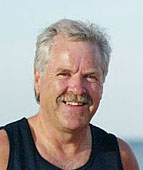
\includegraphics{imgs/houler.jpg}
  \end{center}
  \vspace{-30pt}
\end{wrapfigure}

Houler è un uomo belga di 60 anni, ha una moglie e quattro figli (tre maschi e una femmina, tutti tra gli 8 e i 20 anni). Ha lavorato per oltre 20 anni come fattorino in una PMI di calzature di Monza dove si è trasferito in via stabile all’età di 7 anni. La sua azienda ha chiuso i battenti per bancarotta costringendolo a trasferirsi all’estero, in Romania, dove nelle ultime due settimane ha lavorato come fattorino presso l’azienda Whirlpool. In entrambe le compagnie Houler ha sempre effettuato le proprie consegne con il furgone aziendale dotato di navigatore; sebbene non possa essere considerato un esperto è in grado di utilizzare un computer per visualizzare la posta elettronica, gestire i propri documenti o navigare in internet.

\begin{wrapfigure}{l}{0.4\textwidth}
  \vspace{-30pt}
  \begin{center}
    
\includegraphics{imgs/veronica.jpg}
  \end{center}
  \vspace{-30pt}
\end{wrapfigure}

\newpage

Veronica è una ragazza modenese nubile di 29 anni. E’ fidanzata da dieci mesi con un ragazzo del suo stesso paese due anni più piccolo di lei. Fa volontariato presso l’Ospedale Maggiore di Bologna ed attualmente è alla ricerca di lavoro nella medesima città. Ha appena completato gli studi presso l’università di Scienze Politiche di Modena con ottimi risultati e la sua ambizione più grande consiste nel lavorare per la pubblica amministrazione. Durante gli studi ha sostenuto e superato l’esame per la patente europea ECDL. All’età di 12 anni, essendo andata a visitare i parenti con la propria famiglia in un paesino limitrofo Modena, si perse nella cittadina per oltre 6 ore. Terrorizzata da tale esperienza Veronica odia viaggiare e preferisce di gran lunga la sicurezza della sua città.

\begin{wrapfigure}{l}{0.4\textwidth}
  \vspace{-30pt}
  \begin{center}
    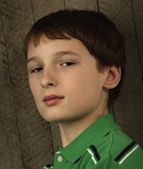
\includegraphics{imgs/franz.jpg}
  \end{center}
  \vspace{-30pt}
\end{wrapfigure}

Franz è un ragazzino tedesco di 12 anni e mezzo. Frequenta la scuola media a Berlino con risultati medio scarsi. Tende a distrarsi facilmente, e per questo motivo ha ripetuto due volte la prima media. I suoi genitori, Daniel e Camille, lavorano entrambi presso la stessa ambasciata, l’uno come ambasciatore, l’altra come inserviente. Franz adora i videogiochi e giocare a pallone con i suoi coetanei nel ruolo di portiere. I suoi genitori tendono a viaggiare molto portandolo con sè, nonostante la sua tenera età ha già visitato decine di città in tutta Europa. La sua tata polacca gli racconta spesso del suo Paese dal quale Franz sembra essere particolarmente affascinato. Una volta l’anno Franz si reca con la mamma ed il papà in Francia dai genitori di lei (i suoi nonni) con i quali comunica principalmente in inglese, lingua che conosce particolarmente bene.

\section{Contesto D'Uso}

\subsection{Caratterizzazione degli utenti}

Al fine di definire con assoluta precisione l’utenza di riferimento dell’applicazione Visual Directions è stato compilato un questionario in 11 punti. I risultati relativi sono riassunti di seguito:

\begin{itemize}
	\item L’utente non necessita di alcuna esperienza pregressa nell’uso di Visual Directions.
	\item L’utente può beneficiare di una conoscenza marginale del prodotto Google Maps (o preferibilmente Google Street View).
	\begin{itemize}
		\item L’utente non deve necessariamente aver utilizzato in precedenza
		\begin{itemize}
			\item Prodotti dotati della stessa interfaccia
			\item Prodotti dotati di interfaccia simile o paragonabile a quella di Visual Directions.
		\end{itemize}			
	\end{itemize}

	\item L’utente non necessita di alcuna formazione mirata all’uso dell’applicazione.
	\item L’utente non necessita di alcuna particolare qualifica per utilizzare l’applicazione.
	\item L’utente deve essere in grado di navigare in internet e compilare form per poter beneficiare dell’applicazione Visual Directions.
	\item L’applicazione non ha requisiti di natura linguistica.
	\item L’età dell’utenza di riferimento è stimata dai 12 ai 70 anni (ed oltre).
	\item L’applicazione può essere utilizzata indifferentemente da uomini e donne.
	\item L’applicazione è indirizzata ai soli utenti vedenti.
	\item Il livello di istruzione richiesto dall’applicazione è la terza media o superiore. Non si esclude che l’applicazione possa essere utilizzata anche da utenti con un livello di istruzione inferiore.
	\item L’utenza di Visual Directions utilizza l’applicazione per scopi personali.
\end{itemize}

\subsection{Caratterizzazione dei task}

Allo stesso modo sono stati analizzati i task degli utenti. Da tale analisi è emerso un solo scopo dominante le cui caratteristiche sono riportate di seguito:

\begin{itemize}
	\item L’obiettivo del task consiste nel memorizzare un percorso stradale all’interno di una città  mai vista in precedenza ed essere poi in grado di orientarsi in essa senza l’ausilio di mappe o altri strumenti.
	\item Il risultato del task è un’immagine mentale del percorso memorizzato.
	\item Il task è episodico, si assume che l’utenza lo effettui occasionalmente.
	\item La durata del task è stimata dai 5 ai 30 minuti.
	\item Decomposizione del task in azioni elementari:
		\begin{itemize}		
			\item Accesso all’interfaccia
			\item Inserimento degli indirizzi di partenza e di destinazione
			\item Visione del percorso
			\begin{itemize}
				\item Fruizione incidentale e/o ripetuta
				\item Memorizzazione del percorso
			\end{itemize}
		\end{itemize}
\end{itemize}

\subsection{Vincoli (tecnici, culturali, ambientali)}

È stato altresì necessario discutere dei vincoli di carattere tecnico, culturale ed ambientale cui gli utilizzatori dell’applicazione sono soggetti. È particolarmente interessante constatare che, sebbene l’applicazione evidenzi svariati vincoli tecnici e culturali sembra essere invece esente da vincoli ambientali. La seguente lista riassume i vincoli rilevati per quanto concerne l’utilizzo dell’applicazione Visual Directions:

\begin{itemize}
	\item Vincoli tecnici
	\begin{itemize}
		\item Al fine di utilizzare l’applicazione è necessario un dispositivo elettronico come un PC, un tablet o uno smartphone. In linea di principio è anche necessaria una connessione ad Internet.
		\item Il sistema non fornisce copertura completa del globo terrestre, pertanto non ogni percorso è visualizzabile.
	\end{itemize}
	\item Vincoli culturali
	\begin{itemize}
		\item L’utente deve conoscenza dei requisiti fondamentali per memorizzare delle informazioni stradali (i.e. prendere appunti su punti di rilievo interessanti) ed orientarsi in ambienti ignoti.
	\end{itemize}
\end{itemize}


%----------------------------------------------------------------------------------------
%----------------------------------------------------------------------------------------

\chapter{Progettazione}

A fronte di una fase di analisi dei requisiti e di progettazione è stato realizzato un prototipo  dell’applicazione Visual Directions per poter valutare l’effettiva efficacia del progetto. I principali risultati di tale operazione che includono i requisiti progettuali, i dettagli implementativi e i limiti del prototipo sviluppato sono oggetto del presente capitolo. 

\section{Requisiti}

Un percorso cela una quantità considerevole di informazioni utili che ne semplificano la memorizzazione. Si considerino ad esempio le “zone dense”, ovvero delle aree ricche di contenuto informativo quali ad esempio agli incroci, le rotonde e le curve strette; in generale tutti luoghi che è importante osservare lentamente, con calma, proprio in virtù del fatto che contengono una mole considerevole di dati da notare e memorizzare. Allo stesso modo si pensi alle “zone sparse”, ossia aree povere di contenuto informativo, come ad esempio i rettilinei, le autostrade e gli ampi viali che richiedono di certo meno lavoro ed attenzione per essere memorizzate.

Un requisito importante dell’applicazione Visual Directions consiste nel rendere semplice ed intuitivo discriminare e memorizzare tanto le zone dense quanto le zone sparse di un determinato percorso. Pertanto l’applicazione calcola automaticamente la velocità con la quale presenta i dati di interesse (i fotogrammi immersivi di street view), basandosi sulle coordinate che sta mostrando in un determinato istante e l’angolo derivante dalle coordinate visualizzate in precedenza o che visualizzerà in futuro.

Un'altro aspetto, particolarmente importante nella visualizzazione Street View, è quello dell'orientamento della camera. Bisogna considerare in modo preciso le parti da visualizzare durante il percorso: quando voltare la camera in prossimità di curve ed incroci, nonchè prevenire o ritardare la rotazione in curve molto poco accentuate.

Allo stesso modo è importante che l’applicazione sia snella e consumi poche risorse (in particolare per quanto riguarda la banda dati e la potenza di calcolo) poichè si suppone che questa venga utilizzata da utenti dotati di computer o altri dispositivi non eccessivamente performanti. 

\section{Prototipo dell’applicazione Visual Directions}

\subsection{Le API di Google Maps}

Al fine di realizzare il prototipo dell’applicazione Visual Directions è stato necessario appoggiarsi ad un sistema esistente per il calcolo delle coordinate geografiche che compongono determinati percorsi e per la resa grafica degli stessi. Il celebre prodotto Google Maps fornisce entrambe tali componenti attraverso una API particolarmente semplice e versatile. In particolare, mediante richieste HTTP di tipo GET è possibile:

\begin{itemize}
	\item Trasformare coppie di indirizzi (sorgente, destinazione) in liste di coordinate geografiche che identificano dettagliatamente un percorso da un punto ad un altro.
	\item Recuperare e visualizzare delle immagini satellitari (con granularità variabile fino al più fine dettaglio stradale) relative ad un punto identificato da specifiche coordinate geografiche ed un particolare angolo di orientamento.
\end{itemize}

\subsection{Implementazione}

L’implementazione del prototipo stante al progetto Visual Directions è stata effettuata a mezzo del linguaggio di scripting javascript, la libreria jQuery, e Google Maps Javascript API v3.

Questa libreria mette a disposizione un servizio importante, chiamato Directions Service, che permette di risolvere query anche piuttosto complesse.

La lista di coordinate geografiche fornite da Google Maps non è di per sé sufficiente per costruire un video di un percorso che sia sufficientemente semplice da fruire. Si pensi ad esempio al fatto che svariati punti forniti dall’API, nei rettilinei, sono piuttosto distanti l’uno dall’altro, mentre nelle zone piene di curve ed incroci sono molto vicini, a volte anche in maniera apparentemente del tutto casuale. Affinché la velocità di riproduzione del video non dipenda dalla distribuzione dei punti nello spazio, occorre filtrarli in maniera opportuna; abbiamo deciso perciò di parametrizzare i punti del percorso, in modo da riuscire a definire una funzione $f(p, s)$ che preso in input un percorso $p$ ed una dimensione spaziale $s$, espressa in metri, riesca a restituire la coordinata geografica situata dopo $s$ metri dal punto di partenza del percorso $p$. In questo modo è possibile riprodurre il video con una velocità costante prefissata, in modo tale da poter muovere il punto di osservazione con velocità espressa in metri al secondo. 

Inoltre, al fine di evitare di fornire troppi dettagli lungo i rettilinei e troppo pochi durante i cambi di direzione, abbiamo deciso di variare la velocità di movimento all’interno del percorso in maniera automatica, in funzione della variazione dell’angolo dato dal punto di osservazione.

Nei dettagli: 

\begin{itemize}
	\item Sia $M$ il numero massimo di metri percorribili durante l’iterazione corrente. 
	\item Sia $\Delta$ la differenza tra l’angolo di osservazione misurato durante l’iterazione corrente e l’angolo di osservazione misurato durante l’iterazione immediatamente precedente.
	\item Il numero di metri da coprire all’interno del percorso durante l’iterazione in oggetto è fissato in: $0 < M * e^{-|\Delta|} \le M$, essendo la funzione esponenziale negativa compresa tra $0$ e $1$.
\end{itemize}
Ciò significa che la velocità di movimento lungo il percorso decresce esponenzialmente in prossimità di curve e/o svincoli che rappresentano verosimilmente i punti più difficili da memorizzare.

Tra l’altro, anche la velocità di refresh dei fotogrammi del video prodotto dall’applicazione dipende dalla variazione dell’angolo di osservazione. È di fatti ragionevole che il video mostri più lentamente una lunga sequenza di fotogrammi relativi a punti geograficamente prossimi gli uni altri altri (esattamente come accade in prossimità delle curve) e più velocemente una più breve sequenza di fotogrammi relativi a punti geograficamente distanti (come accade lungo i rettilinei). 

Chiaramente è stato necessario introdurre una soglia limite al tempo di attesa tra due refresh consecutivi onde evitare che lungo le curve l’utente fosse costretto ad attese eccessive. La formula relativa è la seguente: $min\{ 500, \; 200*e^{|\Delta|} \}$.

\subsection{Considerazioni e limiti del prototipo}

Benchè l’implementazione prodotta sia perfettamente funzionante, è tuttavia soggetta ad una vasta gamma di problemi che la rendono inadatta per l’applicazione estensiva in contesti reali. Tali problemi sono per lo più legati alle limitazioni delle API di Google Maps. Queste infatti non hanno delle primitive sufficientemente avanzate per definire callback che segnalino la fine del caricamento delle immagini, proprio perché sono state pensate per visualizzazioni per lo più statiche. Ne consegue che questo tipo visualizzazioni, che stressano in maniera particolare la banda, e senza la possibilità di costruire opportuni meccanismi che regolino la velocità dei fotogrammi in base alla banda disponibile, possono essere a volte essere frammentarie e confusionarie.

Inoltre, poiché tale servizio non ha ancora a disposizione le immagini in grado di coprire tutto il globo terrestre, è impossibile visualizzare determinati percorsi. Tra l’altro Google permette di effettuare ai propri server solo una quantità limitata di richieste giornaliere a titolo gratuito; ne consegue che attualmente il nostro prototipo non può soddisfare le richieste di una popolazione più ampia del campione di test oggetto dei successivi capitoli.

\subsection{Interfaccia del prototipo}

L’interfaccia dell’applicazione Visual Directions è stata sviluppata ponendo particolare enfasi sulla semplicità d’uso e la praticità. La minimalità è la parola chiave. Come è possibile vedere nelle rappresentazioni (concepts) di seguito, la stessa consta di due form testuali in cui è possibile inserire rispettivamente gli indirizzi di partenza e di destinazione e tre semplici tasti che permettono la manipolazione del video. Il tasto Play permette di avviare la riproduzione del video, il tasto Pause permette di interromperla momentaneamente, il tasto Stop permette di arrestare la visualizzazione del video ed eventualmente cominciarne una nuova. Animate polemiche in merito alle funzionalità del tasto Stop sono state oggetto di studio ed hanno spinto il team di sviluppo a discutere della necessità di modificare il nome di tale pulsante. È stata inoltre introdotta una barra di scorrimento che viene mostrata dopo l’avvio del video che ne permette la riproduzione incidentale.

\begin{figure}[H]
\centering
{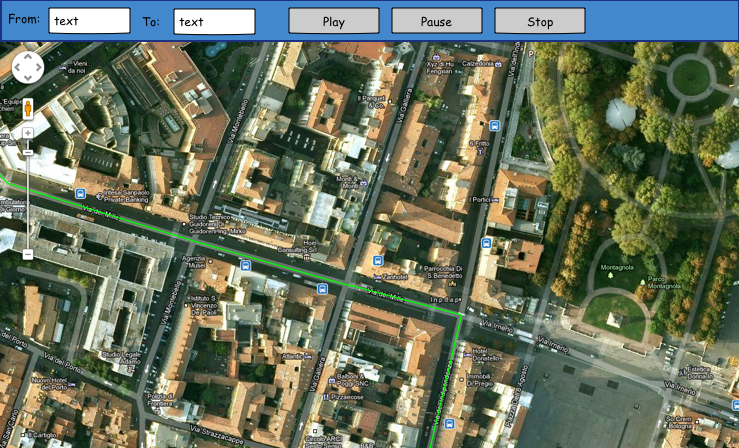
\includegraphics[width=\textwidth]{imgs/prototipe-interface1}}
\end{figure}

\begin{figure}[H]
\centering
{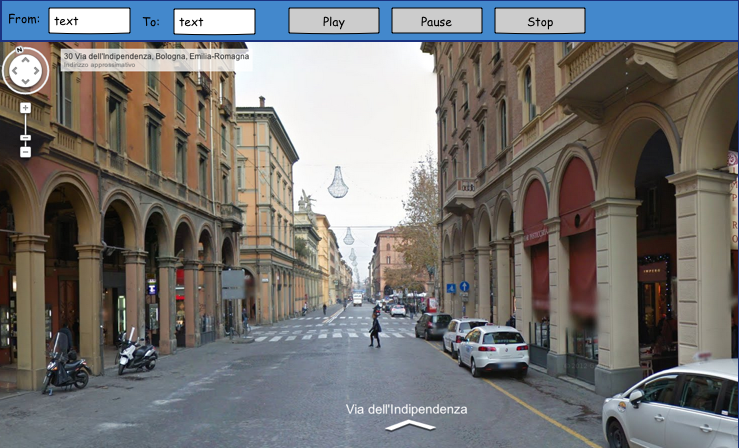
\includegraphics[width=\textwidth]{imgs/prototipe-interface2}}
\end{figure}


%----------------------------------------------------------------------------------------
%----------------------------------------------------------------------------------------

\chapter{Valutazione Interna}

Sulla base del prototipo dell’applicazione discusso in precedenza, del task fondamentale definito nell’ambito del contesto d’uso (memorizzazione di un percorso cittadino), delle azioni elementari che lo compongono e sulla base degli utenti, dei personaggi e delle loro competenze e aspettative, il team di sviluppo ha realizzato una valutazione interna del progetto secondo la tecnica del Cognitive Walkthrough. Ha di fatti individuato una storia rappresentativa del contesto d’uso primario dell’applicazione e ne ha valutato la credibilità evidenziandone problemi e criticità.

\section{Cognitive Walkthrough}

\subsection{Storia}

Alice deve andare a trovare Bob, il quale vive in un’altra città. Alice raggiungerà questa città in treno, ma il suo problema è riuscire ad andare a casa di Bob a partire dalla stazione dei treni di Proserpia Marittima, dove però Alice non ha mai messo piede prima. Nè ha mai visto Bob. Alice non ha un navigatore, né uno smartphone, né una mappa di Proserpia Marittima. Deve pertanto imparare l’intero percorso prima di partire, o quantomeno imparare i punti più importanti del percorso (in modo da poter chiedere informazioni). Quindi, Alice accede alla nostra interfaccia, inserisce il luogo di partenza e arrivo del percorso che dovrà seguire e avvia il video in modalità street-view. Con molta attenzione, memorizza (e se necessario annota) ogni punto di riferimento che ritiene importante lungo il percorso, come ad esempio: punti di svolta; punti di riferimento utili come fontane, farmacie, palazzi, montagne, ecc., che le serviranno per potersi orientare lungo il percorso il giorno in cui dovrà andare da Bob. Infine, il giorno della partenza, Alice arriva alla stazione di Proserpia Marittima, e uscita dalla stazione riconosce subito la strada che deve percorrere. Ad un certo punto si perde, ma chiede informazioni per arrivare ad un punto noto che aveva memorizzato nel percorso (una piazza con un grande orologio ed una statua), riesce quindi a mettersi nella giusta direzione ed arriva da Bob in tempo per l’appuntamento.

\subsection{Valutazione interna della storia}

La storia è stata giudicata abbastanza plausibile da ogni membro del team di sviluppo, eccetto per quanto concerne i problemi qui di seguito elencati.

\subsection{Problemi scoperti}

\begin{itemize}
	\item Assunzioni:
	\begin{itemize}
		\item Non è detto che Alice sia in grado di identificare facilmente quali sono i form da editare per inserire l’indirizzo di partenza, l’indirizzo di destinazione nè quale sia il tasto da premere per avviare la visualizzazione del video del percorso. Ma è plausibile che ci riesca in breve tempo, viste le premesse sul tipo di utenza.
		\item Non è detto che Alice riconosca a prima vista il punto di partenza del percorso da lei visualizzato mediante Visual Directions. Potrebbe darsi che debba girovagare un pò o chiedere informazioni per identificare l’inizio di tale percorso.
	\end{itemize}
	
	\item Differenze tra il modello mentale del progettista e quello dell’utente:
	\begin{itemize}
		\item E’ plausibile che l’utente si aspetti che il video del percorso cominci premendo il tasto \textbf{Invio} dopo aver inserito l’indirizzo di partenza e quello di destinazione. L’interfaccia progettata prevede la necessità di premere il pulsante \textbf{Play} a tal fine.
	\end{itemize}
	\item Etichette:
	\begin{itemize}
		\item Il pulsante \textbf{Stop} blocca la visualizzazione del video relativo al percorso attuale e permette di cominciare la visualizzazione di un nuovo percorso. E’ verosimile che alcuni utenti associno il concetto di Stop a quello di Pause, inducendo in un utilizzo erroneo dell’applicazione.
	\end{itemize}
\end{itemize}

\subsection{Modifiche Proposte}

In seguito ai problemi riscontrati nella fase di Cognitive Walkthrough, sono state individuate le seguenti modifiche progettuali:

Modifica del nome del pulsante \textbf{Stop} in \textbf{Rewind} che chiarisce meglio lo scopo del pulsante stesso.
Introdurre la possibilità di premere \textbf{Invio} dopo aver compilato i form degli indirizzi di partenza e destinazione al posto di premere il tasto Play per avviare la visualizzazione del video.


%----------------------------------------------------------------------------------------
%----------------------------------------------------------------------------------------

\chapter{Test}

\section{Test dell’applicazione Visual Directions}

Il test dell’applicazione Visual Directions è stato orientato a misurare in modo effettivo l’efficienza e l’efficacia della stessa. In termini generali, con il termine efficienza ci si riferisce al tempo impiegato da un utente per raggiungere il proprio obiettivo; con il termine efficacia ci si riferisce invece all’effettivo ausilio apportato dall’applicazione in termini di memorizzabilità dei percorsi visualizzati, ovvero il numero di errori da questi commessi nello svolgimento del test stesso. Il test è stato diviso in due fasi:

\begin{itemize}
	\item \textbf{Osservazione}, durante la quale gli utenti hanno visualizzato due percorsi, uno loro noto in precedenza ed uno non noto, ambedue della lunghezza di un chilometro.
	\item \textbf{Orientamento}, durante la quale gli utenti hanno visualizzato delle immagini (di incroci o altri punti di snodo stradale) ed è stato loro chiesto se riconoscevano tali punti. In caso di risposta affermativa è stato loro inoltre richiesto di indicare in quale direzione fosse necessario continuare per proseguire lungo il tragitto stante alla fase di osservazione cui tale punto apparteneva.
\end{itemize}

\section{Test di osservazione}

Durante la fase di osservazione è stato chiesto agli utenti di visualizzare ogni percorso finchè non avevano la ragionevole certezza di poterlo percorrere a piedi senza ausilio di mappe o ulteriore strumentazione che semplifichi l’orientamento. E’ stato loro permesso di utilizzare l’interfaccia dell’applicazione per muoversi all’interno del percorso in qualsiasi modo ritenessero necessario, attivando tasti e manipolando la barra di scorrimento del video.

Nel caso specifico i percorsi in esame sono riassunti di seguito (i collegamenti ipertestuali agli stessi sono forniti in appendice):

\begin{itemize}
	\item Percorso noto in precedenza
	\begin{itemize}
		\item Della lunghezza di 1.0 Km
		\item Presso la cittadina di Bergen in Norvegia
		\item A partire da Byparken, piazza centrale a Stromgaten, dove è sito uno dei più importanti centri commerciali della città
	\end{itemize}
	
	\item Percorso non noto in precedenza
	\begin{itemize}
		\item Della lunghezza di 1.0 Km
		\item Presso la cittadina di Plzen in Repubblica Ceca
		\item A partire da Rooseveltova a Sady Pětatřicátníků
	\end{itemize}
\end{itemize}

Durante tale fase sono stati raccolti i dati stanti alla seguente lista:

\begin{itemize}
	\item Orario di inizio visualizzazione del primo video
	\item Orario di termine visualizzazione del secondo video
	\item Numero di volte che ognuno dei due video è stato rivisto (in via parziale o totale).
	\item Percentuale del percorso rivisto per entrambi i video.
	\item Dati sensibili relativi agli utenti per indagini a fini statistici.
\end{itemize}

Ai fini di determinare l’efficienza dell’applicativo sono state identificate delle soglie limite prima di effettuare i test. Tali valori sono raccolti nella seguente lista:

\begin{itemize}
	\item La \textbf{confidence speed}, espressa nella forma di metri al secondo è ottenuta dividendo la lunghezza dei percorsi visualizzati (duemila metri) per il numero di secondi che ogni utente ha speso osservando i video prima di dichiarare di essere sicuro di poter proseguire lungo tali percorsi nella vita reale. Tale valore rappresenta a tutti gli effetti la velocità di memorizzazione del percorso (in particolare, quanti metri un utente è in grado di memorizzare efficacemente ogni secondo). Una confidence speed media di 3 m/s sarà requisito irrinunciabile per il superamento del test di efficienza. 
	\item Il test di efficienza sarà ritenuto superato se la media del numero di volte che i percorsi vengono rivisti è inferiore a 3.
	\item Ed infine la media delle percentuali dei percorsi rivisti non deve eccedere il 33%.
\end{itemize}

\section{Test di orientamento}

Per permettere una valutazione oggettiva dell’efficacia del progetto è stato quindi richiesto agli utenti di visualizzare una serie di immagini relative al percorso appena visionato. Per ogni percorso sono state mostrate loro tre coppie di immagini, ogni coppia relativa ad un certo punto appartenente ad una delle due città da cui i video sono stati tratti. Si noti che tali immagini sono state recuperate per mezzo di applicazioni differenti da Google Street-View, onde sottolineare l’ovvio divario tra le immagini virtuali di Visual Directions ed il loro equivalente reale.

Per ogni tripla di coppie, una coppia di immagini ritraeva un punto non appartenente al percorso. Gli utenti non avevano cognizione di tale dettaglio pertanto le loro osservazioni in merito alla riconoscibilità dei punti visualizzati rispecchiavano la difficoltà oggettiva di memorizzazione del percorso. Tra l’altro le immagini relative ai percorsi sono state fornite in ordine casuale al fine di incrementare ulteriormente la difficoltà di associazione dei dati visuali memorizzati (a breve termine) a queste.

Per ogni risposta di ogni utente sono stati calcolati i punti di errore relativi utilizzando la seguente metrica:

\begin{itemize}
	\item Se l’utente non riconosce un punto del percorso matura 4 punti errore
	\item Se l’utente riconosce un punto non del percorso matura 1 punto errore
	\item Se l’utente riconosce un punto ma non sa dove andare matura 3 punti errore
	\item Se l’utente riconosce un punto ma sbaglia direzione matura 2 punti errore
\end{itemize}

Si noti che il presentarsi di un errore esclude tutti gli altri e i punti errore sono attribuiti per gravità crescente. E’ di fatti ragionevole, ad esempio, credere che l’applicazione non sia per nulla efficace se mediamente gli utenti tendono a non riconoscere punti che effettivamente avevano visualizzato. Al contrario è verosimile ed accettabile che un utente ritenga di aver visto un punto non appartenente al percorso in quanto i punti di snodo stradale si assomigliano molto l’un l’altro.

Ne consegue che il miglior risultato possibile è 0. Il peggiore è 18. Ogni risultato è stato quindi normalizzato relativamente al massimo errore possibile al fine di ottenere una misura della percentuale di errore di ogni utente. Il test di efficacia è da ritenersi superato se la media delle percentuali di errore è inferiore a $1/3$.

\section{Risultati dei Test}

I risultati del test sono riassunti di seguito:

\begin{itemize}
	\item La \textbf{percentuale media di errore} ammonta a 0.23 che è effettivamente minore di $1/3$, pertanto tale fase del test è da ritenersi \textbf{superata con successo}.
	\item La \textbf{media delle confidence speed} è 5.84, superiore a 3; anche questa fase del test è stata quindi \textbf{superata}.
	\item La media del numero di volte che un pezzo di percorso è stato rivisto è 1.5, minore di 3. Anche questa fase di test è stata \textbf{superata}. In particolare è stato rilevato che una porzione sensibile del campione di utenza che ha effettuato il test non ha avuto bisogno di rivedere porzioni di percorso in nessuna occasione per padroneggiarlo.
	\item La media delle percentuali del percorso riviste è il 75\%, maggiore del 33\%. Pertanto questa fase del test è stata \textbf{fallita}. Tuttavia è estremamente curioso osservare che tutti i tester che hanno rivisto una porzione del percorso lo hanno effettivamente voluto rivedere per intero (il che giustifica tale risultato). Ciò è probabilmente dovuto alla richiesta di ``rivisualizzare un percorso fino ad essere certi di poterlo percorrere nella vita reale''; è verosimile credere che la natura di questo comportamento sia da ricercarsi in più profonde analisi psicologico-cognitive.
\end{itemize}

Altri dati interessati raccolti sono i tempi medi che ogni utente ha sperimentato per fornire risposte relative alla seconda fase del test. I risultati sono riassunti nella seguente lista ed evidenziano come un utente riesca a rendersi conto in tempi piuttosto brevi di aver perso o meno l’orientamento.

\subsubsection{Tempistiche di risposta}

\begin{itemize}
	\item Non riconosco questo punto del percorso: circa 10 secondi in media.
	\item Riconosco questo punto del percorso: circa 5 secondi in media.
	\begin{itemize}
		\item E devo proseguire in questa direzione
		\begin{itemize}
			\item Ne sono sicuro: circa 5 secondi in media.
			\item Non ne sono certo: anche oltre 20 secondi di riflessione considerando svincoli, semafori e facendo affidamento sulla conoscenza del percorso nel caso del percorso noto.
		\end{itemize}
	\end{itemize}
\end{itemize}

\subsubsection{Osservazioni dei tester}

Sebbene gli utenti che hanno testato l’applicazione si siano constantemente e fermamente lamentati della qualità del video durante la sua riproduzione sono poi riusciti ad ottenere risultati rispettabili nel quiz relativo. 

Una tester ha dichiarato: “Riconosco questo incrocio ma non sono certa che coincida con quello che ho visto nel video perchè non ricordo questo semaforo”. E’ intrigante osservare che le risposte degli utenti sono opera di un più profondo procedimento deduttivo che esula la banale ricerca nella memoria a breve termine. 

Inoltre, a seguito della visualizzazione dei video dei percorsi, i tester si sono mostrati estremamente avviliti nel non essere in grado di riconoscere il primo punto mostrato loro nel quiz (punto che non poteva in alcun modo essere riconosciuto poichè estraneo al percorso in oggetto). Si sono mostrati interessati e felici di essere invece in grado di riconoscere il secondo punto del quiz contro ogni loro precedente aspettativa.

\section{Test dell’applicazione Google Street View}

È stato infine effettuato un test dell’applicazione Google Street View al fine di effettuare un’analisi comparativa di tale prodotto con l’applicazione Visual Directions.

Un campione di tester (differente dal campione che ha testato l’applicazione di cui sopra ma egualmente numeroso) ha acceduto Google Street View nel punto di partenza dei medesimi percorsi descritti in precedenza ed è stato loro permesso di muoversi liberamente attraverso di esso nel tentativo di giungere in una determinata destinazione (anch’essa coincidente con il punto finale del relativo percorso nel test di osservazione dell’applicazione Visual Directions). Quando gli utenti hanno dichiarato di sentirti sicuri di poter raggiungere tale percorso nella vita reale è stato loro proposto il quiz stante al paragrafo “Test di orientamento”.

I risultati sono raccolti di seguito:

\begin{itemize}
	\item La \textbf{percentuale media di errore} ammonta a 0.71 che è decisamente maggiore di $1/3$, pertanto tale fase del test è stata \textbf{fallita}.
	\item La \textbf{media delle confidence speed} è 3.12, superiore a 3; questa fase del test è stata quindi \textbf{superata} (sebbene con un margine trascurabile).
	\item Poichè gli utenti non hanno visualizzato un video non è stato possibile calcolare la media del numero di volte che un pezzo di percorso è stato rivisto. Vale lo stesso per quanto riguarda la media delle percentuali del percorso riviste.
\end{itemize}

In definitiva sui dettagli comparabili delle due applicazioni Visual Directions si dimostra estremamente più indicata per la memorizzazione preventiva di percorsi urbani.


\newpage
\section{Visual Directions - Test}

Look at the video. The test supervisor will show you. \\
You are watching a video about a path. You can watch the video several times. \\
You should watch the video until you feel confident enough to go the path on your own \textbf{in real life}.  \\
Afterwards we will ask you some easy question. \\
You can ask the test supervisor for any question. \\

We ask you some information about you. \\
Its up to you how much information you want to provide us. \\

\begin{itemize}
	\item Sex: 
	\item Age: 
	\item Nationality:
	\item Study field:
\end{itemize}

\subsection{Question 1.1}

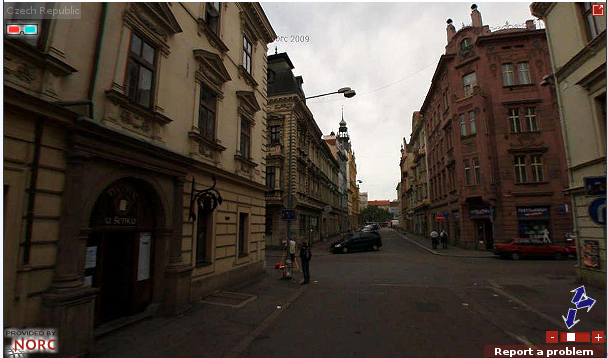
\includegraphics[width=\textwidth]{imgs/image-question11-1}

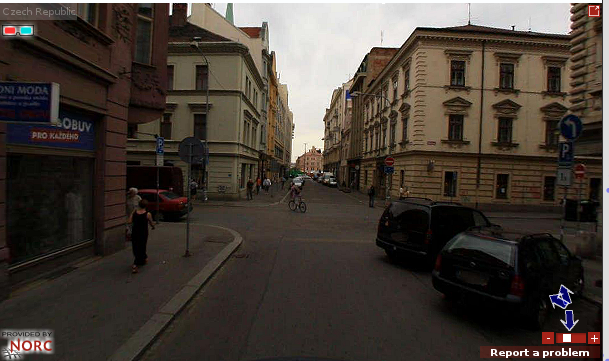
\includegraphics[width=\textwidth]{imgs/image-question11-2}

\begin{itemize}
	\item Do you recognize this point of the city?
	\item If you recognize it, where should you go in order to reach the destination you saw in the video?
\end{itemize}

\newpage

\subsection{Question 1.2}

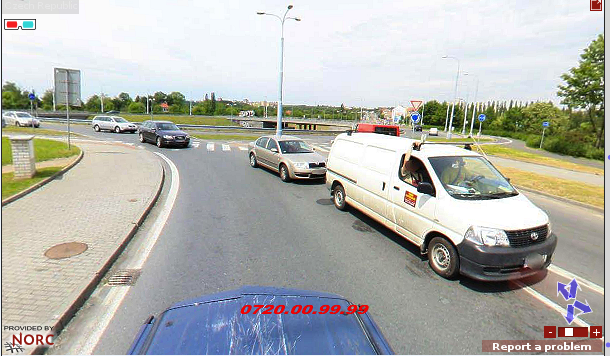
\includegraphics[width=\textwidth]{imgs/image-question12-1}
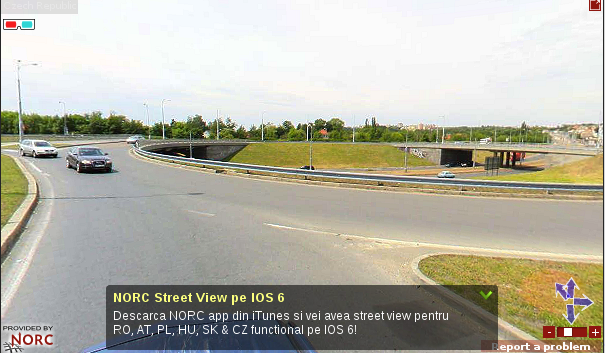
\includegraphics[width=\textwidth]{imgs/image-question12-2}

\begin{itemize}
	\item Do you recognize this point of the city?
	\item If you recognize it, where should you go in order to reach the destination you saw in the video?
\end{itemize}

\newpage

\subsection{Question 1.3}

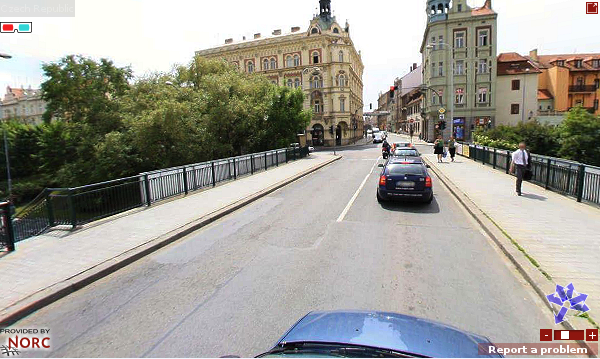
\includegraphics[width=\textwidth]{imgs/image-question13-1}
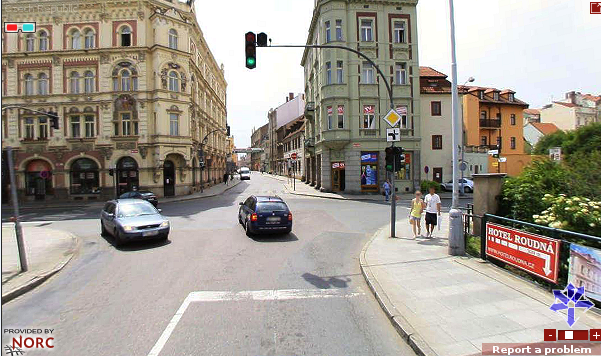
\includegraphics[width=\textwidth]{imgs/image-question13-2}

\begin{itemize}
	\item Do you recognize this point of the city?
	\item If you recognize it, where should you go in order to reach the destination you saw in the video?
\end{itemize}

\newpage

\subsection{Question 2.1}

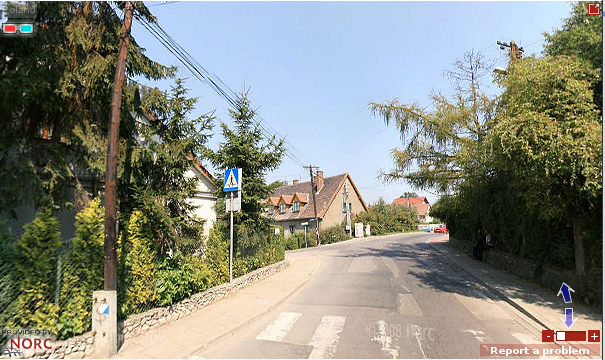
\includegraphics[width=\textwidth]{imgs/image-question21-1}
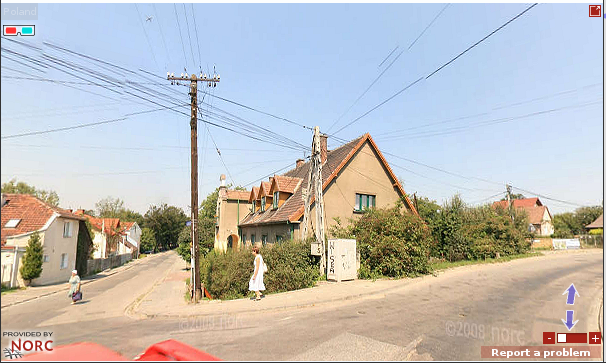
\includegraphics[width=\textwidth]{imgs/image-question21-2}

\begin{itemize}
	\item Do you recognize this point of the city?
	\item If you recognize it, where should you go in order to reach the destination you saw in the video?
\end{itemize}

\newpage

\subsection{Question 2.2}

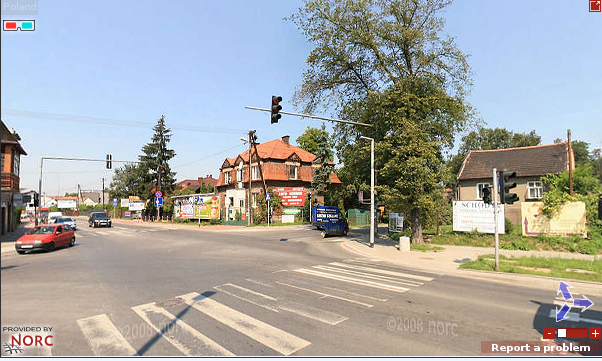
\includegraphics[width=\textwidth]{imgs/image-question22-1}
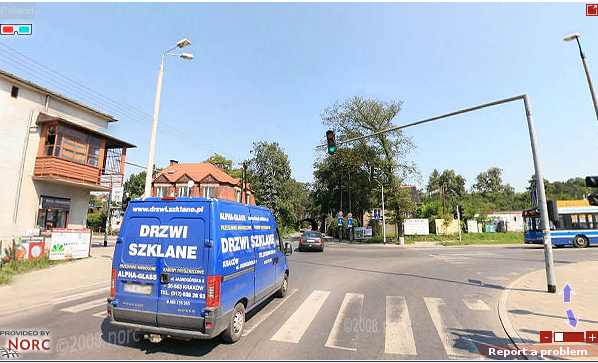
\includegraphics[width=\textwidth]{imgs/image-question22-2}

\begin{itemize}
	\item Do you recognize this point of the city?
	\item If you recognize it, where should you go in order to reach the destination you saw in the video?
\end{itemize}

\newpage

\subsection{Question 2.3}

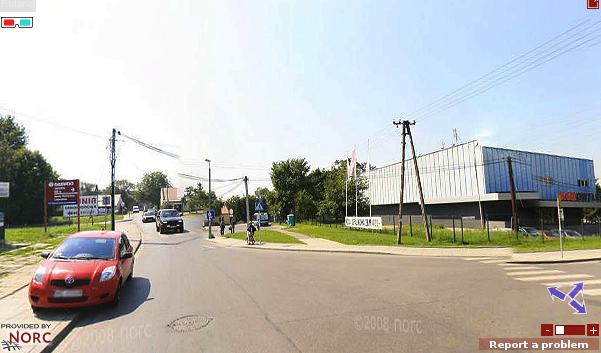
\includegraphics[width=\textwidth]{imgs/image-question23-1}
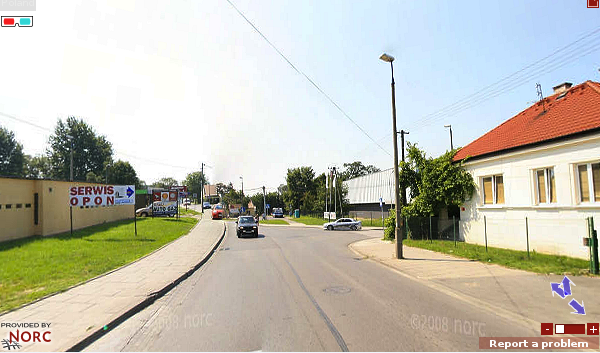
\includegraphics[width=\textwidth]{imgs/image-question23-2}

\begin{itemize}
	\item Do you recognize this point of the city?
	\item If you recognize it, where should you go in order to reach the destination you saw in the video?
\end{itemize}

\newpage

\subsection{Question 3.1}

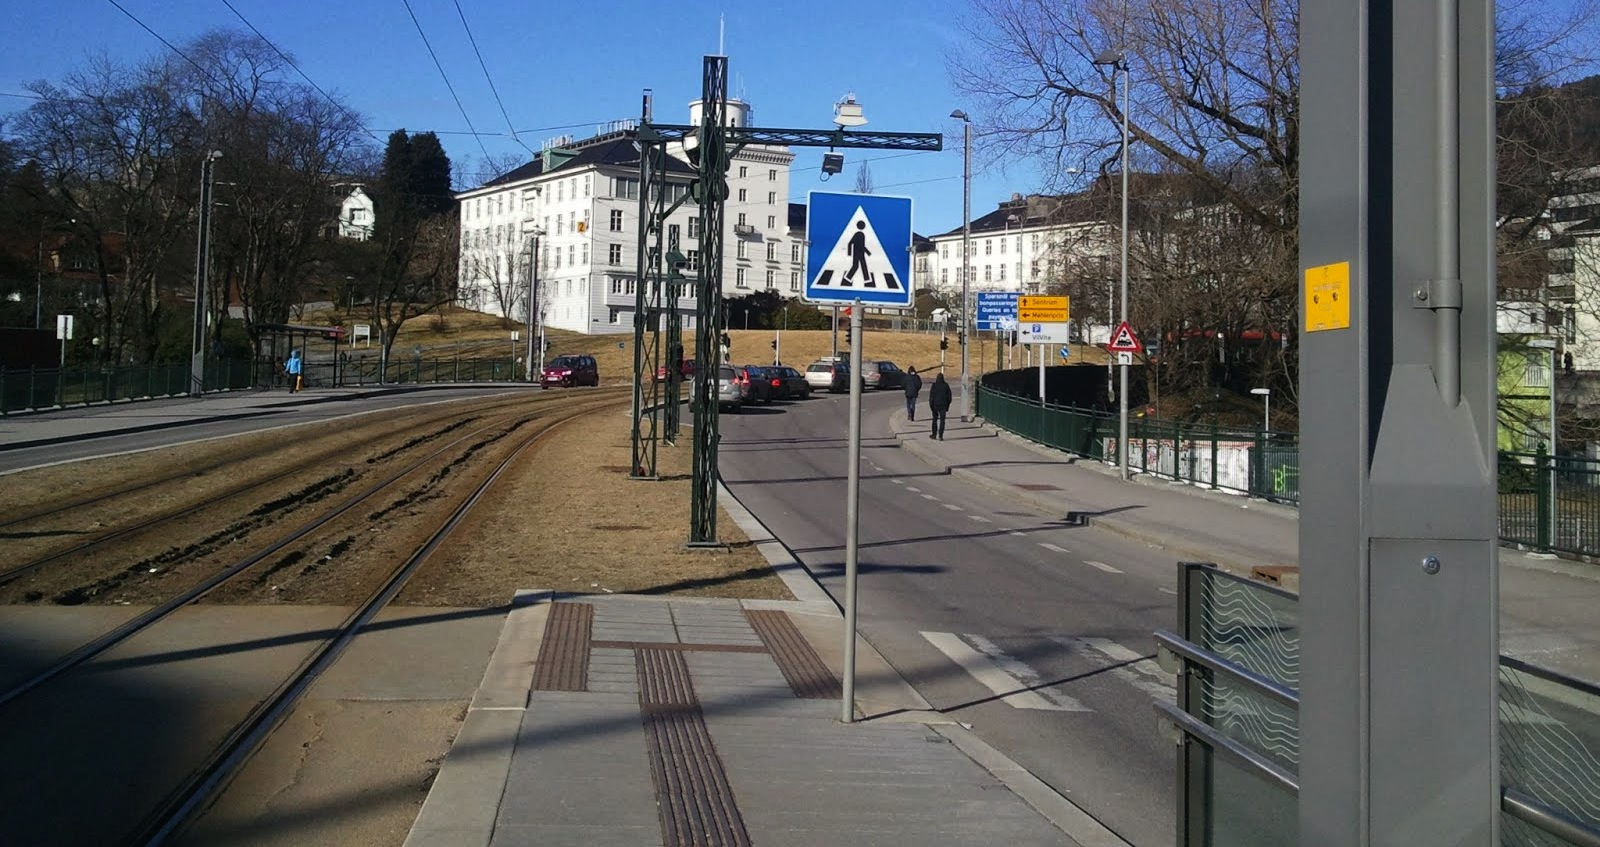
\includegraphics[width=\textwidth]{imgs/image-question31-1}
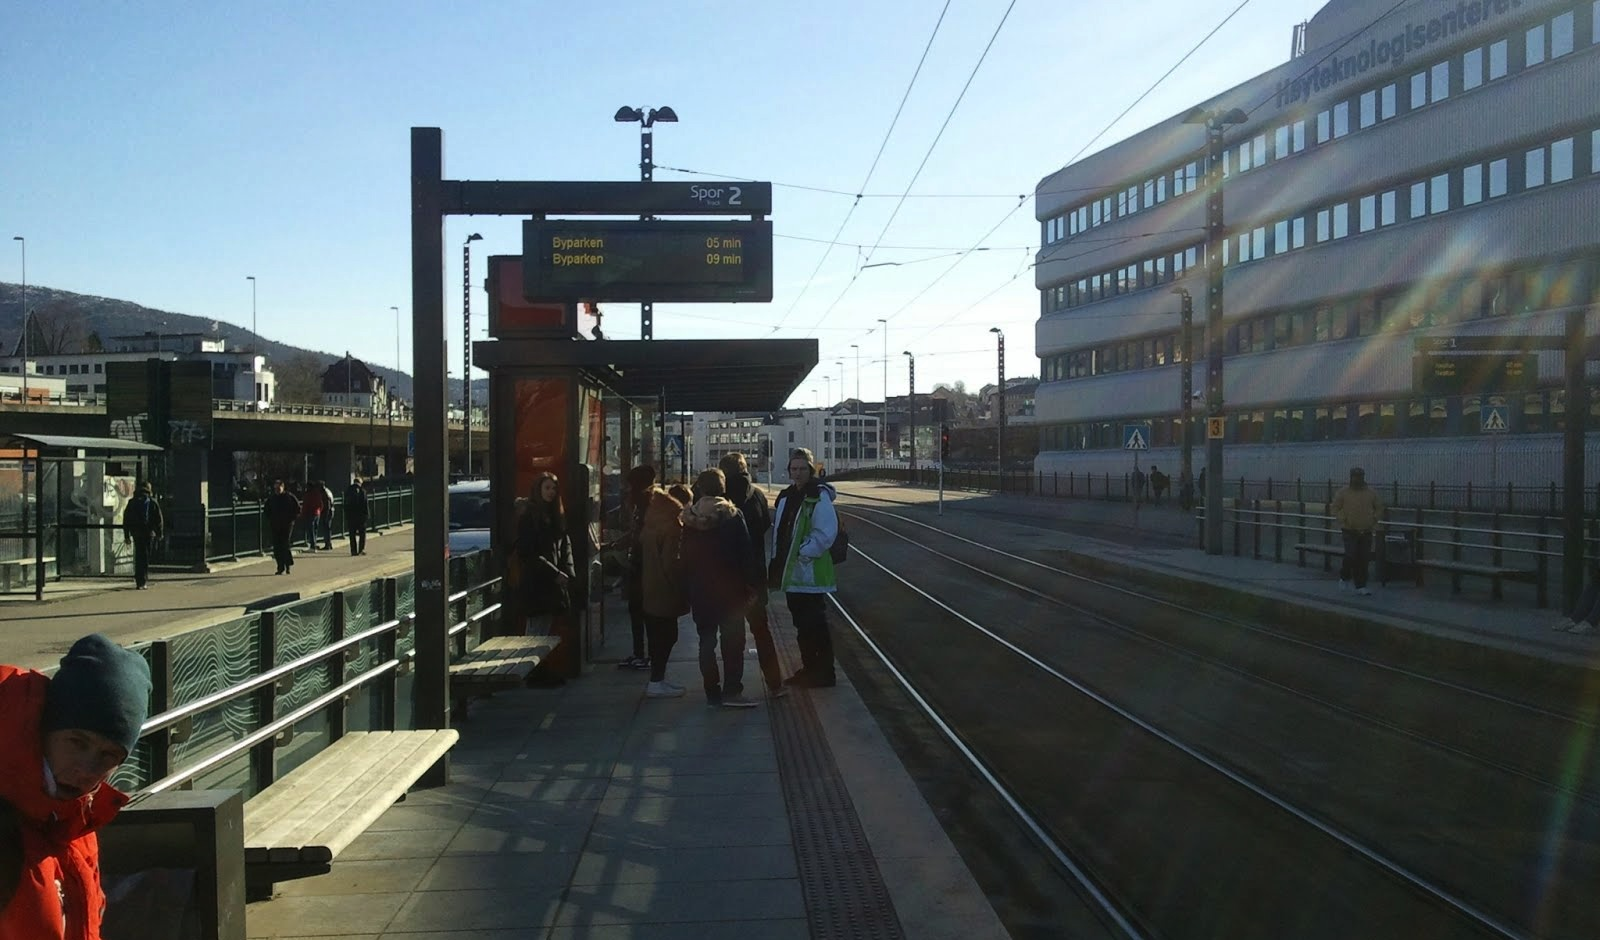
\includegraphics[width=\textwidth]{imgs/image-question31-2}

\begin{itemize}
	\item Do you recognize this point of the city?
	\item If you recognize it, where should you go in order to reach the destination you saw in the video?
\end{itemize}

\newpage

\subsection{Question 3.2}

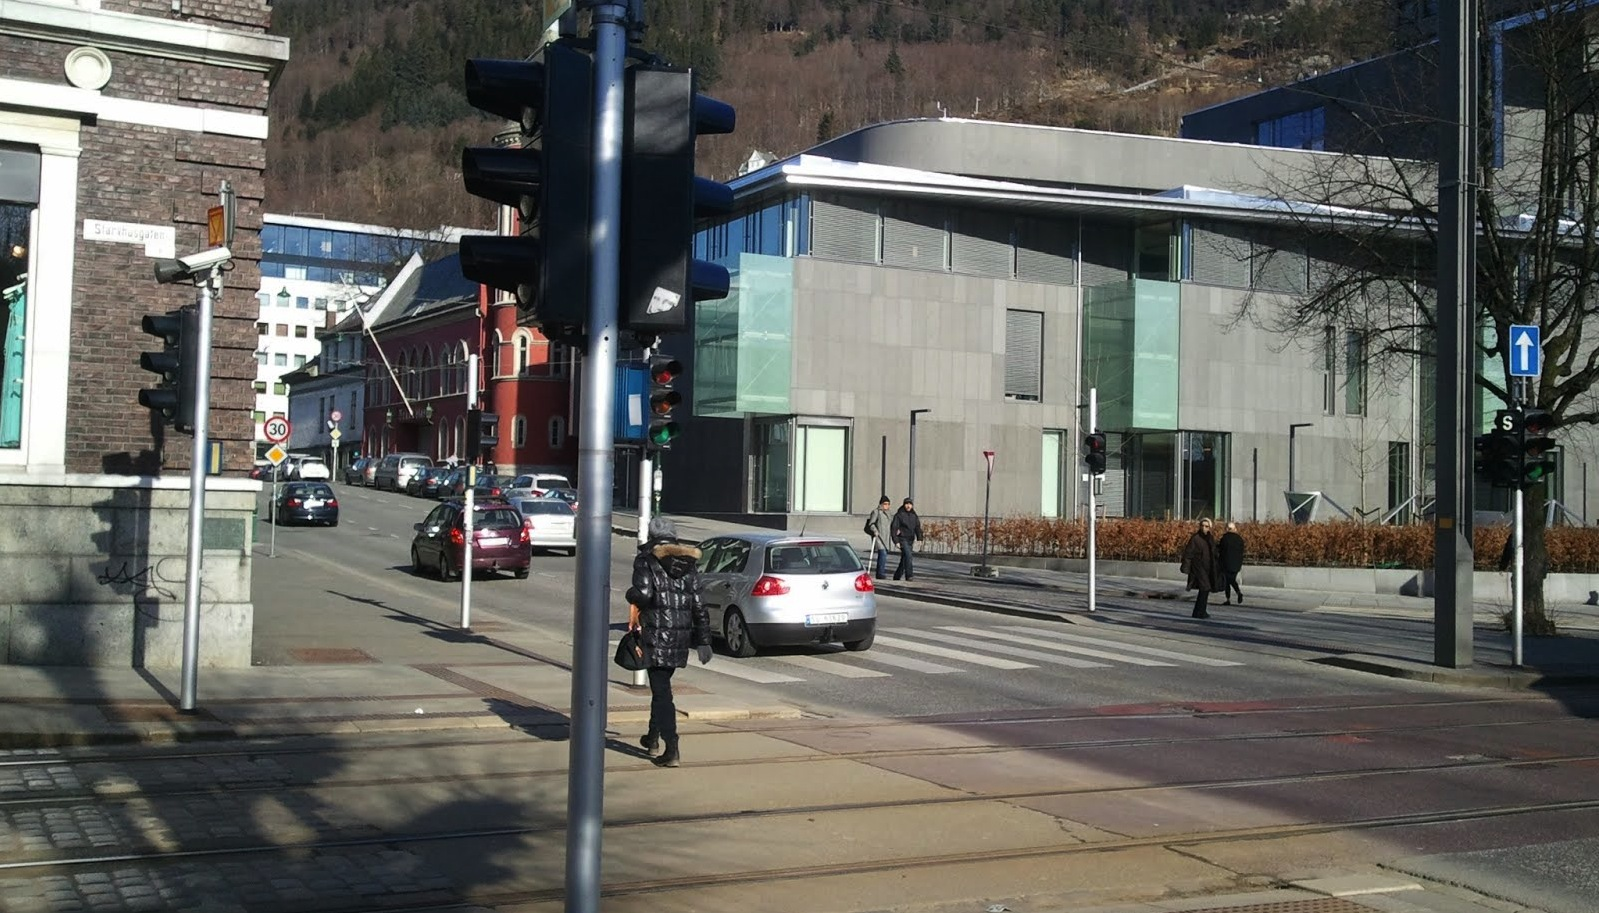
\includegraphics[width=\textwidth]{imgs/image-question32-1}
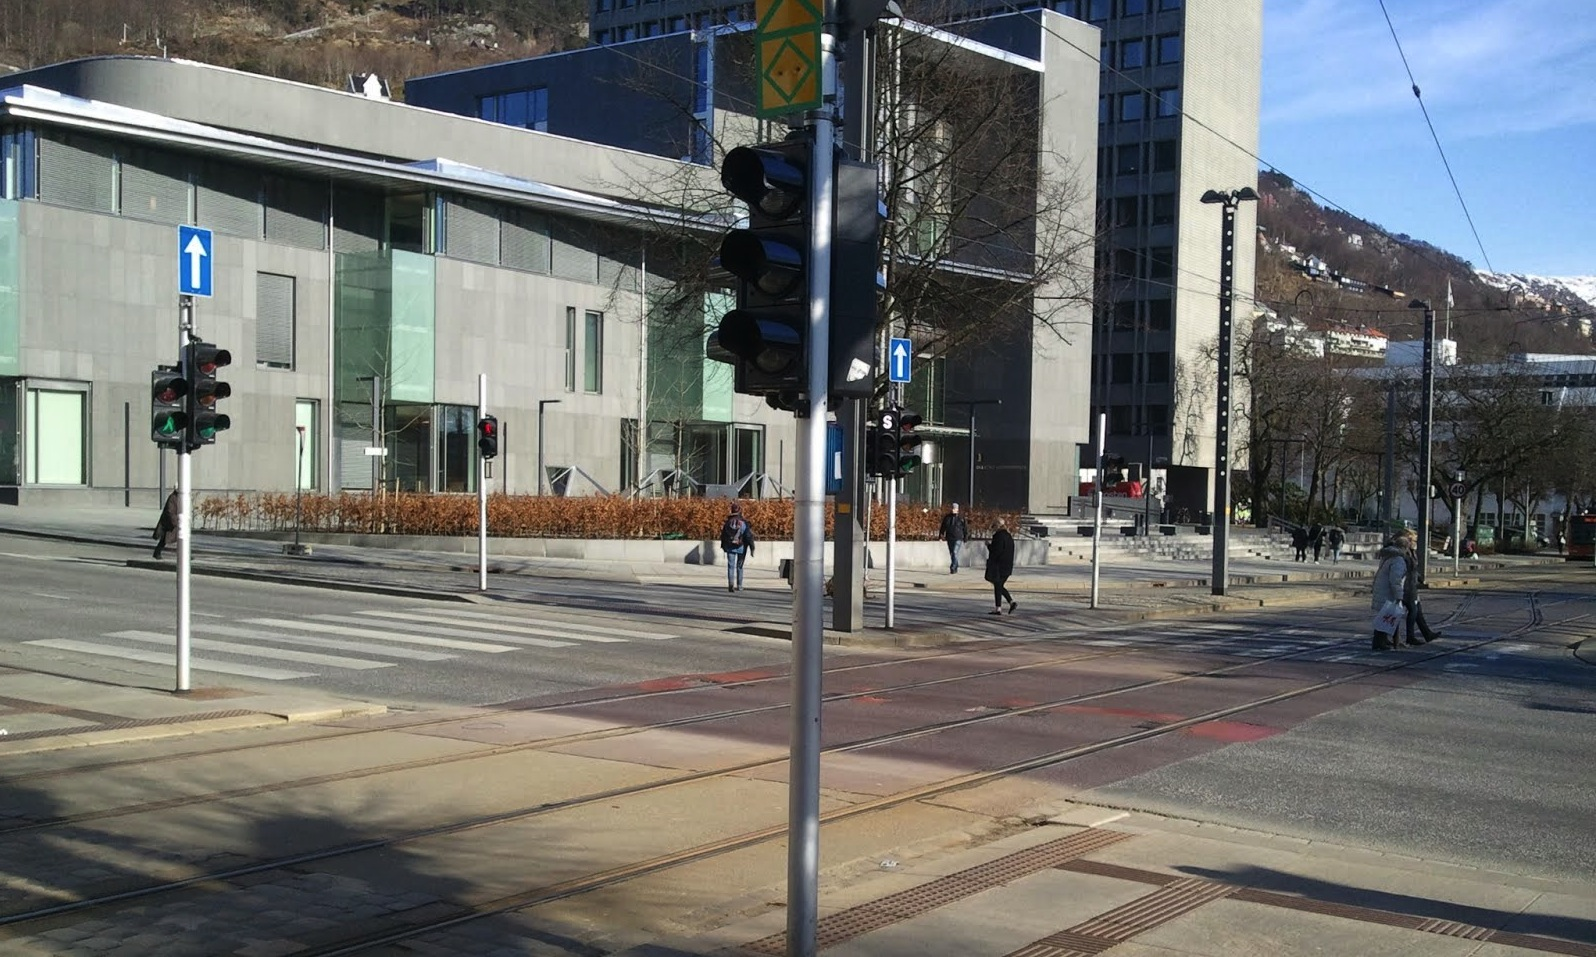
\includegraphics[width=\textwidth]{imgs/image-question32-2}

\begin{itemize}
	\item Do you recognize this point of the city?
	\item If you recognize it, where should you go in order to reach the destination you saw in the video?
\end{itemize}

\newpage

\subsection{Question 3.3}

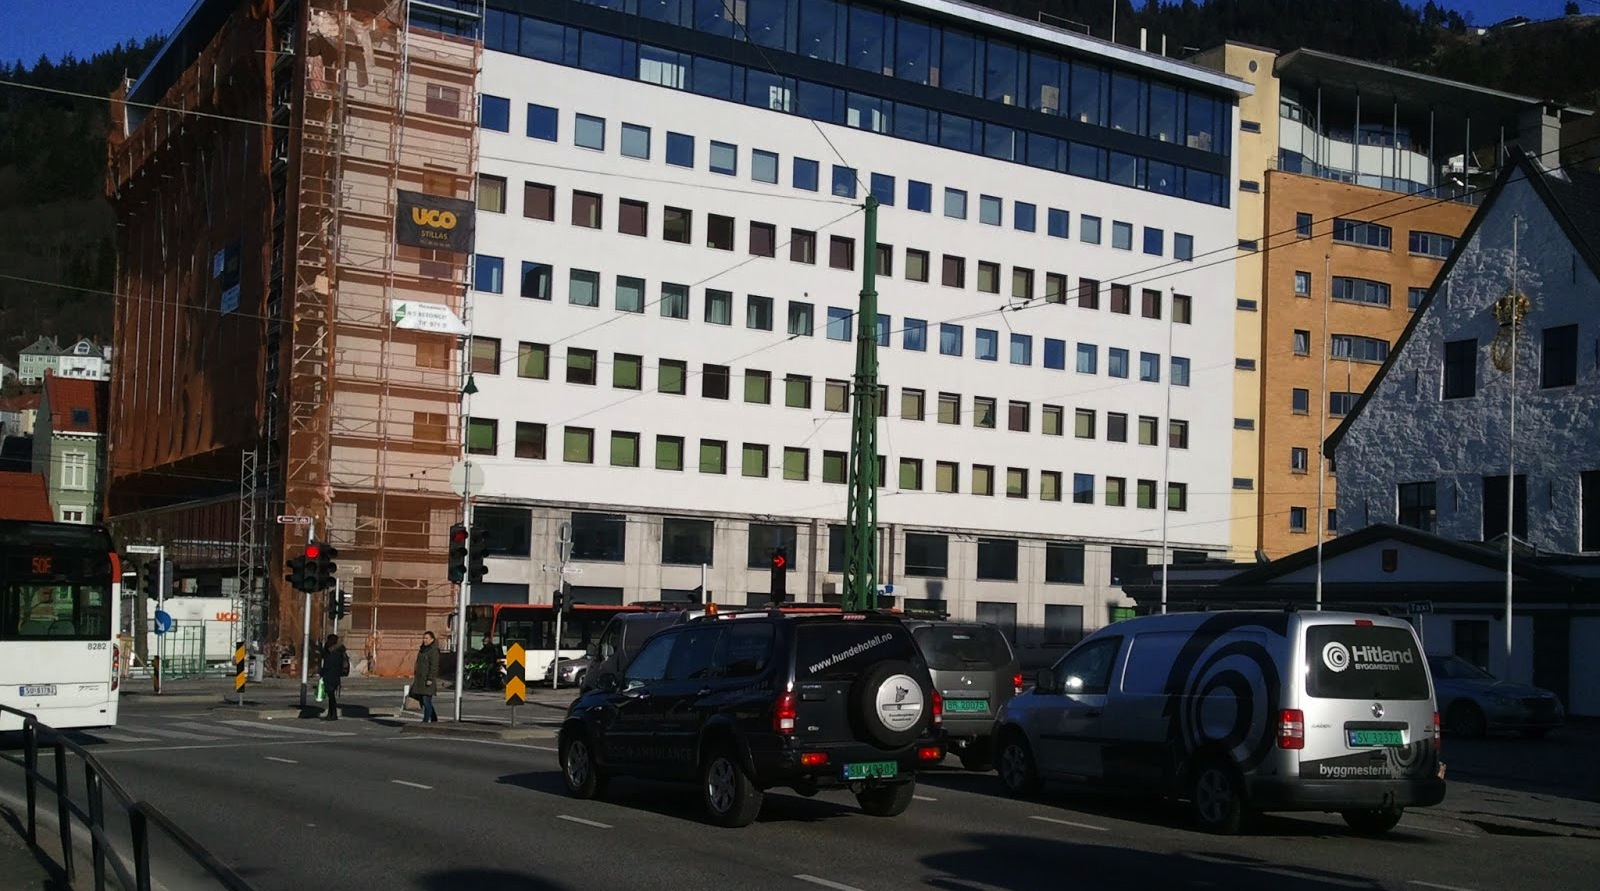
\includegraphics[width=\textwidth]{imgs/image-question33-1}
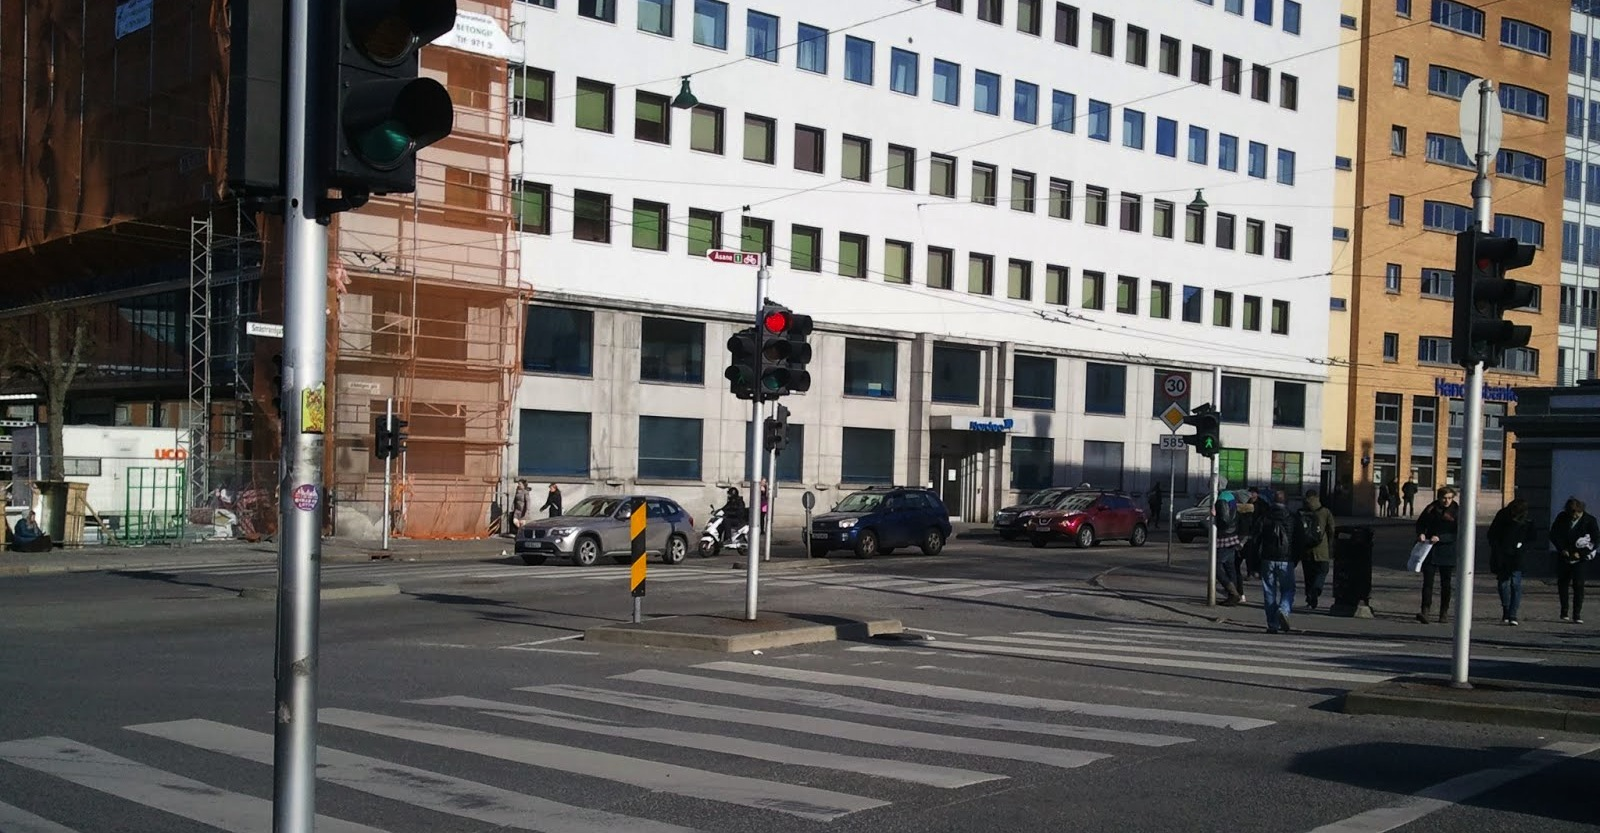
\includegraphics[width=\textwidth]{imgs/image-question33-2}

\begin{itemize}
	\item Do you recognize this point of the city?
	\item If you recognize it, where should you go in order to reach the destination you saw in the video?
\end{itemize}

\newpage


\section{Results}

\begin{adjustwidth}{-1cm}{}
\small
\begin{center}
    \begin{tabular}{| l | l | p{2cm} | l | l | l | l | l | l |}
    \hline
	& 1 & 2 & 3 & 4 & 5 & 6 & 7 & 8 \\ \hline
	starting time & 9:21 & 9:52 & 10:28 & 10:28 & 10:42 & 11:02 & 11:15 & 11:15 \\ \hline
	ending time & 9:34 & 10:01 & 10:32 & 10:32 & 10:50 & 11:10 & 11:23 & 11:23 \\ \hline
	duration & 13 & 9 & 4 & 4 & 8 & 8 & 8 & 8 \\ \hline
	re-watched & 0+1+0 & 2+1 & 0+0 & 0+0 & 0+2 & 1+1 & 1+1 & 1+1 \\ \hline
	% of path reviewed & 100 & 100 & 0 & 0 & 100 & 100 & 100 & 100 \\ \hline
	score & 0.41 & 0.33 & 0.44 & 0.33 & 0 & 0 & 0.11 & 0.22 \\ \hline
	confidence speed & 9.62 & 3.7 & 8.3 & 8.3 & 4.2 & 4.2 & 4.2 & 4.2 \\ \hline
	sex & M & F & M & M & M & F & M & M \\ \hline
	age & 31 & 24 & 21 & 28 & 53 & 21 & 23 & 23 \\ \hline
	nationality & Bangladesh & Czech republic & Spain & Spain & Germany & Spain & Ghana & Spain \\ \hline
    \end{tabular}
\end{center}
\normalsize
\end{adjustwidth}

Commenti relativi alla prima parte (visualizzazione del video):

\begin{itemize}
	\item Il video è troppo frammentario, è impossibile da capire
	\item Oddio, dove sono finito? (in risposta ad un fotogramma erroneo lungo il percorso)
\end{itemize}

Commenti relativi alla seconda parte (compilazione del test):

\begin{itemize}
	\item Mi sembra di aver visto questa strada ma non ne sono sicuro.
	\item Ricordo questo incrocio ma non mi ricordo di questo semaforo, non sono sicuro che sia lo stesso incrocio che ho visto nel video.
\end{itemize}

\appendix

\chapter{Link}

Collegamenti al prototipo del progetto Visual Directions: 

\url{http://visualdirections.altervista.org}

\begin{itemize}
	\item Bergen, da Byparken a Stromgaten \\
	\url{http://goo.gl/maps/pOn1u}

	\item Plzen, da Rooseveltova a Sady Pětatřicátníků \\
	\url{http://goo.gl/maps/Xx28t}
\end{itemize}

Collegamento all’applicazione concorrente di Google Street-View da cui sono state prelevate le immagini per i test: \url{http://www.norc.ro/street-view/}



%Bibliografia%---------------------------------------------------------------
\bibliographystyle{unsrt}
\addcontentsline{toc}{chapter}{\refname}\nocite{*}
\bibliography{text}
%----------------------------------------------------------------------------

\end{document}